
Concept acquisition is a key and widely studied aspect of human daily cognition \cite{cohen2005handbook, ashby2011human}. Many researchers have claimed that a coding system and a set of rules underlie some of our  abilities to acquire concepts \cite{nosofsky1994rule,tenenbaum2011grow,maddox1993comparing}, and it has been observed that we seem to learn concepts of objects with more ease when there are `simpler' rules that can explain those groupings \cite{shepard1961learning, nosofsky1994comparing, rehder2005eyetracking, lewandowsky2011working,feldman2000minimization,blair2003easy,minda2001prototypes}. 


In the real-world, humans learn concept descriptions while simultaneously deciding on which features to attend \cite{schyns1998development}; and the selected set of features usually determines the structure and complexity of the minimal rules that can describe the concept. For example, the concept \textit{dog} can be explained as {\em a four-legged pet that is not a cat} or as {\em an animal for hunting, herding, pulling sledges or company}. Both descriptions are fully compatible with the concept \textit{dog}, but our experience induces us to choose different relevant features to define the concept. While the first description of {\em dog} could be very well be given by a child having a dog at home, the second could be given by a shepherd or perhaps an ethologist. It is likely that the features used to describe {\em dog} by each agent allows them to compactly describe the concept, while simultaneously separating it from other concepts frequently encountered in their environment. Here, we ask about which features participants use to describe concepts, depending on the logical structure of the description using those features and also on their exposure to previous concepts. Why will someone use {\em cat} or {\em hunting} to define {\em dog}?

\begin{figure}
\begin{center}
	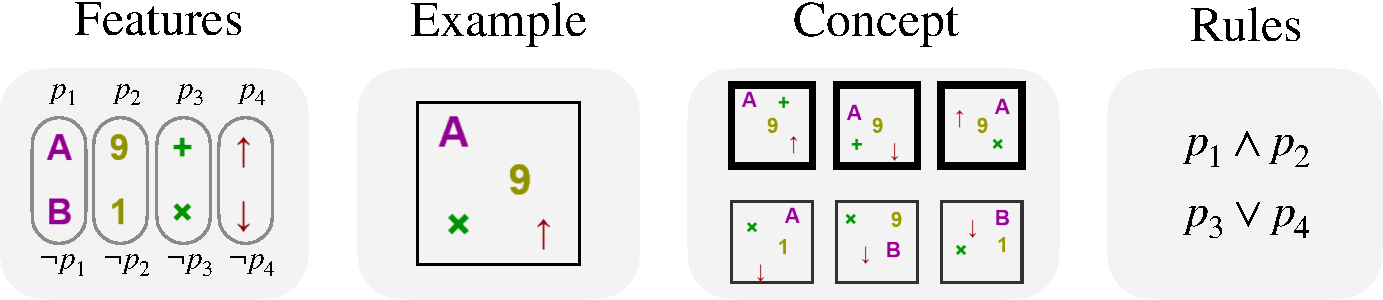
\includegraphics[scale=.6]{Images/intro_notation.pdf}
\end{center}\caption{Illustration of the features $\{p_1,p_2,p_3,p_4\}$, the example $(1,1,0,1)$, and a concept (positive example are marked with bold boundaries and negative examples with thin boundaries). The concept can be explained with the two minimal rules $p_1 \land p_2$ or $p_3 \lor p_4$, depending on which features are used to build the rule (the first two features or the last two features, respectively).}
\label{fig:intro_notation}
\end{figure}



In propositional concept-learning experiments, participants are presented with a set of \textit{examples}, each conformed of $N$ propositional \textit{features}, which can take positive or negative values. For instance, for $N=4$ one example can be logically represented as the element $(1,1,0,1)$, which takes positive values for the first, second and fourth features and negative for the second one, as illustrated in Figure~\ref{fig:intro_notation}. A \textit{concept} can be intuitively understood as a set of examples, some of them marked as belonging to the concept and the rest marked as not belonging, i.e.\ positive and negative examples. In Figure~\ref{fig:intro_notation} we show an example of an \textit{underdetermined} concept, in the sense that, since the entire universe of examples is not shown (i.e. the $2^4$ possibilities), different determined concepts can be consistent with this smaller set when extending the set of examples to the full universe. 

A \textit{rule} consistent with the concept is a logical formula built with the features and the conjunction ($\land$), disjunction ($\lor$), and negation ($\lnot$) operators, which evaluates to true for objects belonging to the concept and false otherwise (e.g.\ $p_1 \land p_2$, where $p_i$ is the $i^{th}$ feature, see Figure~\ref{fig:intro_notation}). The \textit{minimal description length} (\textit{MDL}) of a concept is the length of the shortest rule consistent with the concept \cite{grunwald2007minimum} (here, the {\em length} of a formula is defined as the number of positive or negative occurrences of propositional symbols plus the number of occurrences of operators $\land$ or $\lor$ contained in it; for example, the length of $p_1 \land \lnot p_3$ is 3, and the length of $(p_1 \land \lnot p_3)\lor p_2$ is 5). Importantly, most studies of subjective difficulty with concept-learning are designed such that a {\em single} minimal rule can be used to describe the concept (e.g.\ $p_1 \land p_2$) \cite{ashby2005human,feldman2000minimization}, even when the difficulty of finding the features that compose that rule ($p_1$ and $p_2$) is measured with attention-tracking mechanisms (e.g.\ \cite{blair2009extremely,hoffman2010costs}). This limitation is possibly due to the prohibitively large number of rules that can be built with a given set of features, making it difficult to control which rules the participant might use when observing a set of examples. For instance, in order to determine the difficulty that participants have in learning the logical rule $p_1 \lor p_2$, it is crucial to control that no other rule of reasonable complexity can explain the concept (e.g.\ $p_1 \land p_3$). In this work, we use the tools of propositional logic to build an experimental framework that allows us to present examples consistent with two (or more) chosen rules, depending on which features are observed. For instance, the concept shown in Figure~\ref{fig:intro_notation} is consistent with the explanation $p_1 \land p_2$ \textit{and also} with the explanation $p_3 \lor p_4$, depending on which features are observed. In general, the experimenter can choose any pair of rules that use any number of (non-overlapping) features, and our framework guarantees that the presented examples are only consistent with the two minimal rules chosen by the experimenter. Then, by presenting novel examples that are consistent with only one of the previous rules, the experimenter can determine which rule the participants internally used to learn the concept, and thus which features they attended to.

Presenting rules $A$ and $B$ (e.g.\ $p_1 \land p_2$ and $p_3 \lor p_4$) using the same set of examples has several experimental advantages over separately presenting a set of examples consistent with rule $A$ and then a set of examples consistent with rule $B$. Some of the advantages are: 


\begin{enumerate}
\item [(1)] When comparing the relative difficulty of learning $A$ and $B$ in the same participant, presenting the examples separately makes it hard to overcome transfer effects that cause subjective difficulty to depend on the history of concepts learnt previously in the task, and cause different relative difficulties if $A$ is learnt before $B$ compared to $B$ being learnt before $A$ (see for example \cite{tano2020towards}). The experimenter could compare learning times for $A$ and $B$ across participants, but for reasonably hard rules there are very large idiosyncratic differences in learning difficulties which greatly increases the variance of learning times (see for example \cite{feldman2000minimization}), and also the experimenter cannot normalize the past history of each participant before the experiment. On the other hand, presenting $A$ and $B$ simultaneously via the same set of examples allows us to directly measure which of the two rules is most easily found by the participant, when the two are presented under exactly the same experimental conditions.
\item [(2)] The fact that rule $A$ is learnt more easily than $B$ when presented separately does not necessarily mean that the same happens when presented jointly. This could not hold if there is an interaction between the logical operators being learnt (that compose the rules $A$ and $B$) and the search mechanism used to find the corresponding rules. For instance, the search mechanism that allows humans to find a disjunction rule consistent with the examples could interact with the mechanism that allows to find conjunctions, an interaction that could only be characterized when the conjunction and disjunction are presented at the same time.
\item [(3)] Our framework allows us to test second-order subjective difficulty effects (e.g.\ rule $A$ is learnt faster if presented jointly with rule $B$ than with rule $C$), as well as second-order transfer learning effects (e.g.\  participants learn more rapidly rule $C$ if they have first observed rule $A$ jointly presented with an arbitrary rule $B_1$, compared to $A$ coupled with a different rule $B_2$).
\item [(4)] If one is interested in which features are preferentially observed by the participant in a given trial (e.g.\  features $\{p_1,p_2\}$ or $\{p_3,p_4\}$), one could simply choose the same logical structure for $A$ and $B$ (e.g.\ making $A$ and $B$ equal to $p_1 \land p_2$ and $p_3 \land p_4$) and test whether $A$ or $B$ is learnt by the participant. Then, any preference for learning $A$ over $B$ could only be due to a preference over the features themselves ($\{p_1,p_2\}$), and not for the logical description of the concept using those features (this is, $\boldsymbol{\cdot} \land \boldsymbol{\cdot}$).

\end{enumerate}



We illustrate these advantages in an experiment in which participants are presented with a sequence of 6 trials, observing in each trial a set of examples consistent with two alternative rules. We illustrate advantage (1) and (2) discussed above by presenting a conjunction together with a disjunction; and a simple rule together with a complex rule. Then, we show that after observing in several trials that a subset of features is useful to find concise rules, we induce  in the participants a bias to preferentially describe concepts using those features; this bias was tested exploiting  advantage (4).




